
\chapter{Concepts, nomenclature and definitions in high energy physics (17/11/2016)}

\section{Experimental}

\begin{easylist}[itemize]
\ListProperties(Style*=-- , FinalMark={)})

& Jet: when a quark is produced in a collision, it hadronizes (to become colour-neutral). So another quark is created to pair with the lone quark. But because the particle typically has a lot of energy, more quark-antiquark pairs are produced (the same as when a quark pair is pulled apart, the stored energy in the flux tube between them allows the pair production of quarks, such that there are now two pairs of quarks). This cascades and several quark pairs are produced rapidly, turning into a jet (as each new pair produced travels in the same direction as the original quark(s)).

& $b$-tagging: when bottom ($b$) quarks are produced in accelerator collisions, they hadronize and form jets. The hadrons composed of $b$-quarks have a relatively long lifetime and decay in the detector (or decay between the primary vertex -- initial interaction point -- and the detector to create a second jet and a secondary vertex). Because $b$-quarks have a large mass, their decay products tend to have a high \pt. This leads to high-multiplicity, wide jets. These properties allow the jets to be "tagged" and identified, which can be useful when studying specific decays that would likely produce $b$-quarks.

& Pseudorapidity: the pseudorapidity $\eta$ is a spatial coordinate that describes the angle of a particle (after a collision in an accelerator) relative to the beam axis. The formula is $\eta = -\ln[\tan(\theta/2)]$, where $\theta$ is the angle between the particle's three-momentum and the positive direction of the beam axis. So as $\theta \rightarrow 0^{\circ}$ (the beam line), $\eta \rightarrow \infty$. Generally, particles with large $\eta$ escape the detector (because they are travelling so close to the beam line), so cuts on the order of $|\eta| < 5$ or tighter are usually applied during analysis.

& \alphat: the kinematic variable \alphat is used in analyses to suppress QCD backgrounds, and to suppress multijet production and mis-reconstructed \pt. It is defined in~\cite{Randall:2008rw}, and further described in~\cite{PhysRevLett.107.221804}. Another form is

\begin{equation}
\alphat = \frac{ \sum_{i \in \mathrm{jets}} E_{\mathrm{T}}^i - \Delta E_{\mathrm{T}} } {2 \sqrt{ \left( \sum_{i \in \mathrm{jets}} E_{\mathrm{T}}^i \right)^2 - (\mht)^2 } }
\label{eq:alphaT}
\end{equation}

"where $E_{\mathrm{T}}^i (\equiv E^i \sin\theta^i)$ is the jet transverse energy, and $\Delta E_{\mathrm{T}}$ is the difference in $E_{\mathrm{T}}$ of the two \emph{pseudo-jets}, two sets of jets into which the jets in the event are combined so as to minimize $\Delta E_{\mathrm{T}}$"~\cite{Sakuma:2016nxo}.

& Parton Distribution Function (PDF): a parton distribution function details the momentum distribution of the partons (quarks and gluons) within a proton. There exist many PDFs, that depend on factors such as the energy and the processes that are occurring. See \url{http://www.scholarpedia.org/article/Introduction_to_Parton_Distribution_Functions} and~\cite{Placakyte:2011az}.

& MiniAOD: mini-analysis object data (miniAOD) is a data format used to store data for CMS analyses, and so called because it dramatically reduced the size of the data files. This meant that computing resources and disk space became less strained. See~\cite{1742-6596-664-7-072052} for more information.

& LHE: The Le Houches Accords was an agreement between particle physicists that standardised the interface between the matrix element programs (e.g., \madgraph) and the event generators (e.g., \PYTHIA) used to calculate different quantities. Events that conform to the formats described in the Les Houches Accords are said to be in the Les Houches Event (LHE) format.

& Loose/medium/tight lepton: this type of identification of a lepton refers to the "working points" (cuts) that are applied. The "tighter" the particle, the more (numerous and/or restrictive) cuts are applied. This leads to a lower cut flow efficiency but more accuracy. Usually, the more problems that backgrounds pose, the tighter the cuts are made in order to suppress them. See \url{https://twiki.cern.ch/twiki/bin/viewauth/CMS/SWGuideMuonIdRun2#Muon_Identification} and \url{https://twiki.cern.ch/twiki/bin/viewauth/CMS/CutBasedElectronIdentificationRun2#Electron_ID_Working_Points_WP_de} for more information.

& Control region: orthogonal to the signal region, so no signal is expected. Control regions are used to see if backgrounds are well understood. So you form a "background-only" hypothesis (i.e., no signal -- in the case of Higgs boson searches, the hypothesis would be that $pp$ collisions would produce everything we've seen previously in colliders with no hint of a Higgs, because we hadn't detected the Higgs yet) and predict what your data \emph{should} look like in the regions that aren't the signal region. Then if your data in the control regions agree with your background-only hypothesis, you can build confidence that you're estimating the backgrounds correctly and not introducing any unexpected bias.

& PromptReco and ReReco: % FIND DEFINITIONS

& $\Delta R$: the variable $\Delta R$ is a measure of the angular separation between particles. It is commonly used to define how isolated a particular particle is by constructing a cone of radius $\Delta R$ (the apex of the cone being at the main interaction point, i.e., the primary vertex), calculated via

\begin{equation}
\Delta R = \sqrt{(\Delta\eta)^2 + (\Delta\phi)^2}
\label{eq:deltaR}
\end{equation}

A value of $\Delta R = 0.4$ is commonly used for lepton (namely muon) isolation. Whilst most people say that it isn't a "cone", it's more like a cone in 3D space but a circle in the $\phi-\eta$ plane (which is how the trigger crystals and towers are arranged).

& Isolation/isolated lepton: particle isolation is defined by the fractional momentum contribution of other particles "near" the particle you're interested in. First the track of the target particle is identified. Then a cone of radius $\Delta R$ is constructed (with $\Delta R = 0.4$ being a common choice for muons) around a point in the track with its apex at the primary vertex, and the sums of the \pt and $E_{\mathrm{T}}$ of all the particles within this cone are calculated. Then by dividing by the target particle's \pt you can calculate the fraction of the momentum that other particles are contributing to the total momentum inside the cone, which is also called the value of the particle's "relative isolation". Then you can impose cuts on these values, depending on how isolated you want a certain particle to be.

& Drell-Yan processes: in the LHC, the Drell-Yan (DY) process is when a quark from one proton annihilates with an antiquark from an oncoming proton. This normally produces one of the electroweak bosons, which decays into a lepton-antilepton pair. Looking at invariant mass plots from DY can show clear peaks at the masses of different particles, like the $\phi$. $J/\psi$, $\upsilon$ hadrons and the $Z$ boson. However, as protons contain many quarks, antiquarks and gluons, DY is normally messy and the final states can include several jets.

& \biasedDPhi: the variable \biasedDPhi, known as "biased delta phi", is used in making event selections in signal/data, similar to \alphat~\cite{CMS-PAPER-SUS-15-005-arXiv}. It is based on the minimum azimuthal separation between a jet and the negative vector $\vec{p}_{\mathrm{T}}$ sum of all of the other jets in the event. So it is essentially the minimal separation between the jet and the \htmiss\ vector. It is calculated with the formula

\begin{equation}
  \Delta\phi^*_{\mathrm{min}} = \min_{\,\forall\, \mathrm{j}_k\,\in\, [1,\njet]}
  \Delta\phi \Bigl( \vec{p}_{\mathrm{T}}^{\ \mathrm{j}_k}, \,
    -\hspace{-0.5em}\sum_{\substack{\mathrm{j}_i= 1 \\ \mathrm{j}_i \ne \mathrm{j}_k}}^{\njet}
\vec{p}_{\mathrm{T}}^{\ \mathrm{j}_i} \Bigr).
\label{eq:biasedDPhi}
\end{equation}

& Heavy flavour dark matter: these models include dark matter production in conjunction with heavy-flavour SM particles (top and bottom quarks). The final state products that could be detected would be those quarks (or their decay products) and \etmiss from the DM. Examples of these models can be found in~\cite{Sirunyan:2017xgm}. In contrast, "light flavour" dark matter models yield a final state of dark matter particles and light quarks, i.e., up, down, charm, and strange.

& Systematic uncertainties: systematics are due to uncertainty from known sources. In particle physics analysis, these are from Monte Carlo statistical uncertainties, initial state radiation (ISR), jet energy corrections (JECs), etc., and need to be taken into account because they can affect the reliability of results.

& Look-elsewhere effect: % ADD HERE

& Particle Flow: the reconstruction algorithm used by CMS. It essentially takes the elements (hits, clusters, tracks, etc.) from the different parts of the detector (tracker, ECAL, HCAL, etc.) and correlates them to build up the reconstructed event. See~\cite{CMS-PRF-14-001} for more information. 

& Pileup: in colliders like the LHC, where the proton beams are split into bunches, there is an expected number of collisions/events per bunch crossing at a detector. If there are more than expected, these excess events are deemed as "pileup". At higher luminosities, more pileup events are expected, and so experiments have to find a way to sort the recorded objects correctly to determine which particles came from which event.

& Jet seed: the point of local maximum in a trigger tower (TT) sliding window of some size (currently 9x9 TT in CMS). The trigger tower with the largest energy deposit in the window is used as the seed (the centre of the jet), where the isolation is set by the size of the window. A jet seed threshold is usually applied to prevent recording numerous low-energy/pileup jets. Online Level-1 jets from data are clustered using this method.

& Trigger menu: the collection of trigger algorithms available in firmware at a given time.

& AK4 and AK8: the "AK" stands for "anti-$k_{\mathrm{T}}$", which is a jet clustering algorithm widely used in data analysis from hadron-hadron collisions~\cite{Cacciari:2008gp}. The 4 and 8 give the size of the jet ($R = 0.4$ and $R = 0.8$, respectively). In analyses, people sometimes refer to "AK4" or "AK8" jets, which are essentially jets clustered using the anti-$k_{\mathrm{T}}$ algorithm with the respective $R$ value. So a larger $R$ jet would be more inclusive if you have, say, a fat jet, but the isolation would be worse. This algorithm is used to cluster offline jets (Calo/PF/Gen).

& \etmiss\ vs. \htmiss: \etmiss\ (or MET) is the missing transverse energy, i.e., the negative vector sum of the transverse energies of \emph{all} particles in an event. \htmiss\ (or MHT) is the negative vector sum of the transverse energies (or momenta) of \emph{only the jets} in an event. An easy way to distinguish is to think of the "H" in MHT standing for "hadronic".

& Skimmed and slimmed trees: a skimmed tree is one in which events have been removed that, for example, fail certain cuts. A slimmed tree is one where branches or leaves have been removed, i.e., redundant leaves that contain unnecessary information can be stripped to reduce the size of the tree.

& Monte Carlo truth level: "truth" level in MC refers to particles produced at the generator level, i.e., the base Feynman diagrams. Monte Carlo events are produced by creating the process/decay in a generator like MadGraph. These events are then hadronised and run through a detector simulation. Those two latter steps can potentially cause problems or issues, so sometimes it's better to look at the particles at the generator level and figure out what's going on. Trees with MC events usually store the gen. particle information so it's not too difficult to access.

\end{easylist}

This list will be updated whenever I encounter a new definition and so isn't representative of my knowledge at the time this section was first written (17/11/2016). Some of these explanations are pulled directly from Wikipedia (or have been worded a bit differently than the Wikipedia entry). A glossary of acronyms and various terms in CMS, computing, and high energy physics in general can be found at \url{https://twiki.cern.ch/twiki/bin/view/CMSPublic/WorkBookGlossary}.

As an aside, below is a cross section of CMS. It's useful for scale and to see the tracks of particles.

\begin{figure}[H]
\centering
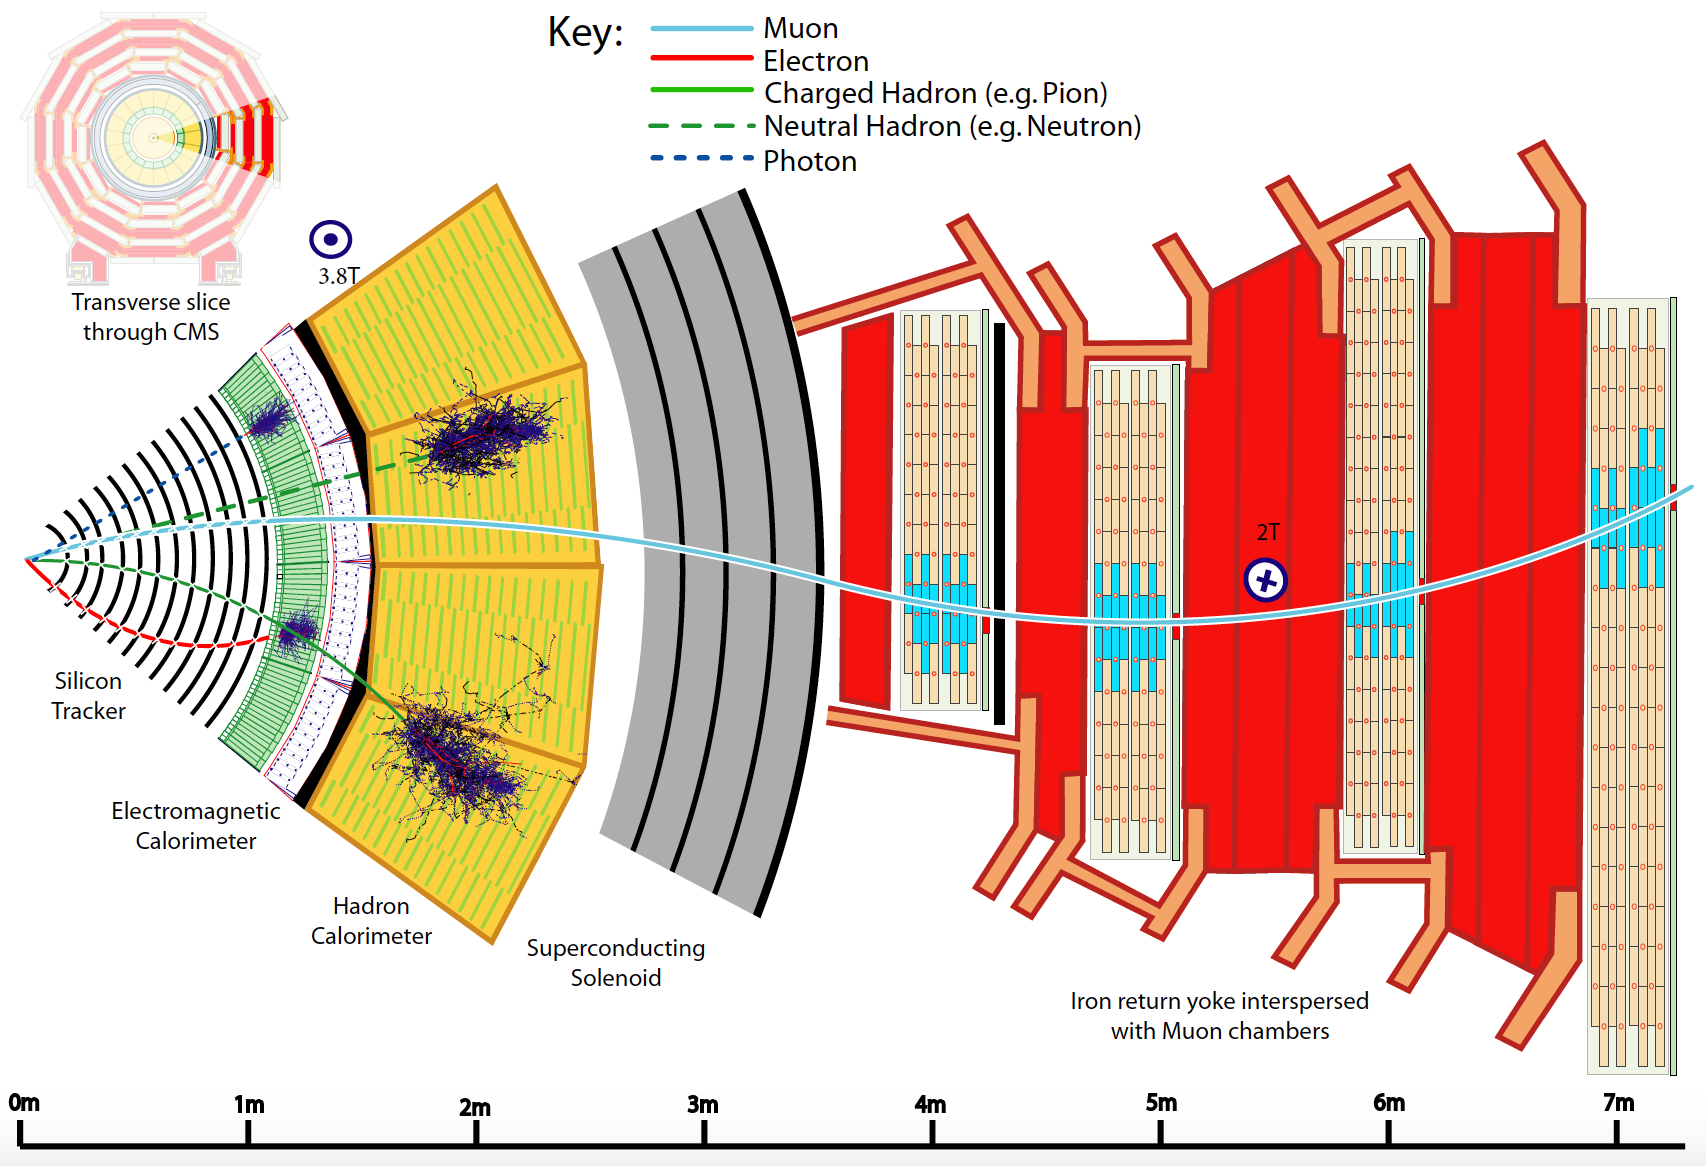
\includegraphics[width=\textwidth]{./sec14/Transverse_slice_CMS.png}
\caption{A transverse slice through CMS, taken from~\cite{CMS-PRF-14-001}.}
\end{figure}

%---------------------------------------------------------------------------------------------------------------

\section{Theoretical}

\begin{easylist}[itemize]
\ListProperties(Style*=-- , FinalMark={)})

& Spinors: vector-like mathematical objects. In particle physics, spinors are associated with the spin of a particle. In QED and QCD, an object formed of two 2-component spinors (effectively spin-up and spin-down states) are solutions to the Dirac equation. For example, the spinor $u_r (\mathbf{p})$ is a positive energy fermion solution of the form

\begin{equation}
u_r (\mathbf{p}) = \mathcal{N}
\begin{pmatrix}
\chi_r \\
\frac{ \boldsymbol{\sigma} \cdot \mathbf{p} }{ E + m } \chi_r \\
\end{pmatrix}
\end{equation}

in compact notation. $\mathcal{N}$ is a normalisation factor, $\boldsymbol{\sigma} = (\sigma_1, \sigma_2, \sigma_3)$ are the Pauli matrices, and $\chi_r$ ($r = 1, 2$) are two-component spinors that cover the spin degrees of freedom for fermions:

\begin{equation}
\chi_1 = 
\begin{pmatrix}
1 \\
0 \\
\end{pmatrix}
\textrm{ and } \ 
\chi_2 = 
\begin{pmatrix}
0 \\
1 \\
\end{pmatrix}
\end{equation}

See~\cite{Steane:2013wra} for more information.

& Tree level: the process that contributes most to an interaction in a Feynman diagram. There are no loops or extra virtual particles created. It is the simplest interaction; most Feynman diagrams you see describing a specific interaction is shown at tree level.

& Loop level: this is one level deeper when looking at an interaction in a Feynman diagram. When looking at loop level, extra virtual particles are created and destroyed (in a loop). For example, in the Lamb shift -- where the 2$s$ and 2$p$ energy levels in hydrogen aren't exactly degenerate as they should be -- is due to the photon (mediating the interaction between the proton and electron) pair-producing two particles that distort the atomic potential and then annihilate to reform the original photon. This is an example of a one-loop effect.

& Yukawa coupling: used in the Standard Model to describe the coupling between a scalar and Dirac field. In the Standard Model, these can correspond to the interaction of the Higgs field with massless quark and lepton fields (i.e., the fundamental fermion particles). Through spontaneous symmetry breaking -- due to the minimum of the Higgs potential being non-zero -- these fermions acquire a mass proportional to the vacuum expectation value (vev, $v$) of the Higgs field:

\begin{equation}
m_f = \frac{y_f v}{\sqrt{2}}
\end{equation}

where $f = l, q$ and $m_f$ is the pole mass.

& On-shell and Off-shell: particles that satisfy classical equations of motion -- such as the action, Euler-Lagrange equations, and Einstein energy-momentum relationship -- are called "on-shell". These include real exchange particles, and any regular, detectable particles. Virtual particles do not obey the above equations and so are considered "off-shell".

& Covariant and contravariant: a contravariant vector is denoted with superscript indices (think "co$\uparrow$travariant"), and its components transform in the same way as the coordinates but in the opposite way to the reference axes. Examples include position, velocity, and acceleration. A covariant vector is denoted with subscript indices (think "co$\downarrow$ariant"), and its components transform in the opposite way as the coordinates but in the same way as the reference axes (i.e., scales with the coordinate system). An example is the gradient of a scalar field.

& Types of vector indices: Greek indices ($\mu$, $\nu$, etc.) are used to denote the components of a 4-vector, while Roman indices ($i$, $j$, etc.) denote the components of spatial 3-vectors.

& $\partial_{\mu}$: this is the four-gradient used in tensor calculus. The operator is a four-vector, and so the result of using it on a variable gives a four-vector. As usual, $\mu = 0, 1, 2, 3$. From Wikipedia,

\begin{equation}
\frac{ \partial }{ \partial X^{\mu} } = \left( \frac{1}{c} \frac{ \partial } { \partial t }, \vec{\nabla} \right) = \left( \frac{ \partial_t }{c}, \vec{\nabla} \right) = \partial_{\mu} = \ ,_{\mu}
\end{equation}

The d'Alembertian,

\begin{equation}
\Box = \partial^{\mu} \partial_{\mu} = \frac{ \partial^2 }{ \partial t^2 } - \vec{\nabla}^2
\end{equation}

& Why the weak force is "weak": this is due to the Higgs field. In the very early universe ($\mathcal{O} (10^{-12}) $ seconds), the Higgs field introducing mass to elementary particles broke a symmetry in the electroweak interaction (before, all particles, including the weak bosons, were massless). When the $W^{\pm}$ and $Z$ bosons gained mass, their force-carrying ability became constrained by the Heisenberg Uncertainty Principle. As the particles mediating an interaction are virtual, they draw from the vacuum energy and so must "pay it back" in a time dictated by the Principle. The weak bosons are very massive, so require a lot of energy for them to pop into existence. And as they can only travel so fast, this limits both the range and strength of the weak interaction.

& Conservation laws as a consequence of symmetries: % ADD

& Quark confinement: single free quarks are never observed because of gluon-gluon interactions. This causes the field to concentrate into a flux tube connecting the quarks within a hadron. The tube stores potential energy and has an associated tension. If the quarks move further apart, the force stays roughly constant but the potential energy (force $\times$ distance) increases linearly with distance. When the potential energy is great enough, the flux tube spontaneously produces a quark-antiquark pair to leave two hadrons.

& Negative energy solutions to Dirac and Klein-Gordon equations: positive energy solutions are just positive energy particles moving with time. Negative energy solutions can be interpreted as negative energy particles moving backward in time, or positive energy antiparticles moving forward in time (because $e^{ -i (-E) (-t) } = e^{ -iEt }$).

& Gamma matrices: the gamma matrices are a component of the Dirac equation, which in itself is a generalisation of the Klein-Gordon equation that fixes some of its problems. These matrices ($\gamma^i$ for $i = 0, 1, 2, 3$) are Hermitian, Traceless (where the sum of the elements on the leading diagonal is zero), and have eigenvalues of $\pm 1$. They are normally written as 2x2 matrices, but each of these elements is itself a 2x2 matrix, i.e.,

\Deactivate % So I can use the ampersand symbol without it starting a new entry in the list or erroring

\begin{equation}
\gamma^0 =
\begin{pmatrix}
\mathbb{1} & 0 \\
0 & \mathbb{-1} \\
\end{pmatrix}
=
\begin{pmatrix}
1 & 0 & 0 & 0 \\
0 & 1 & 0 & 0 \\
0 & 0 & -1 & 0 \\
0 & 0 & 0 & -1
\end{pmatrix}
= \mathrm{diag}(1, 1, -1, -1)
\end{equation}

The next three are defined as

\begin{equation}
\gamma^i =
\begin{pmatrix}
0 & \sigma_i \\
-\sigma_i & 0 \\
\end{pmatrix}
\textrm{for $i = 1, 2, 3,$ where $\sigma_i$ are the Pauli matrices}
\end{equation}

For example,

\begin{equation}
\gamma^1 =
\begin{pmatrix}
0 & \sigma_1 \\
-\sigma_1 & 0 \\
\end{pmatrix}
=
\begin{pmatrix}
0 & 0 & 0 & 1 \\
0 & 0 & 1 & 0 \\
0 & -1 & 0 & 0 \\
-1 & 0 & 0 & 0
\end{pmatrix}
\end{equation}

There is also a fifth gamma matrix $\gamma^5$, which is useful when discussing the chirality of particles. It is defined as

\begin{equation}
\gamma^5 = i \gamma^0 \gamma^1 \gamma^2 \gamma^3 =
\begin{pmatrix}
0 & 0 & 1 & 0 \\
0 & 0 & 0 & 1 \\
1 & 0 & 0 & 0 \\
0 & 1 & 0 & 0
\end{pmatrix}
\end{equation}

which, as well as having the same properties, anticommutes with the other four gamma matrices.

\Activate % Re-activate the ampersand symbol to begin new list entries

& Handedness of particles: the \textbf{helicity} of particles can be thought of as either "left-handed" or "right-handed", which is determined by the alignment of the directions of its spin and motion (linear momentum). If the direction of a particle's spin is the same as the direction of its momentum, the particle is said to be right-handed. If they are opposite, the particle is left-handed. % how to get direction of spin?

For massive particles -- which must always travel below $c$ -- it is possible for an observer to boost into a reference frame where it overtakes the particle. In this case, before the observer overtakes, the particle's helicity will appear one way. But then once overtaken, the particle's helicity will be reversed because the direction of its momentum relative to the observer will be reversed. For massless particles -- which always travel at $c$ -- there is no reference frame in which its helicity can be reversed.

And so, for massless particles its helicity is fixed and therefore Lorentz invariant. For massive particles, helicity can change and so the property of \textbf{chirality} is needed. For massless particles, chirality is the same as helicity. But for massive particles, chirality is the Lorentz invariant property. For a Dirac fermion, it is defined by the $\gamma^5$ matrix operating on the particle's wave function. The chirality can be either left- or right-handed, but is fixed, regardless of reference frame. Chirality is important as the weak force only couples to left-handed fermions and right-handed antifermions (which violates parity).

& Hermitian conjugate: applies to matrices. The Hermitian conjugate of a matrix (usually denoted $A^{\dagger}$ ) is found by taking its complex conjugate and then transposing it. So, $A^{\dagger} \equiv A^{*T}$. If a matrix is labelled "Hermitian", $A^{\dagger} = A$.

& Unitary matrix: a matrix is "unitary" if its Hermitian conjugate equals its inverse, i.e., $A^{\dagger} = A^{-1}$.

& Special group: in group theory, a group is labelled "special" if the matrices within it have a determinant of $+1$.

& $Z$ boson and photon as mixed states: in the GWS model, the electroweak force (before symmetry breaking) contained four massless bosons ($W^+$, $W^-$, $W^0$ and $B^0$). The two neutral bosons mixed to give rise to the $Z^0$ and $A$ (photon) with

\begin{equation}
Z^0 = W^0\cos(\theta_W) - B^0\sin(\theta_W), \ 
A = W^0\sin(\theta_W) + B^0\cos(\theta_W)
\end{equation}

where $\theta_W = 28.7^{\circ}$ is the weak mixing angle, or Weinberg angle.~\cite{tagkey1984quarksandleptons}

& Kaluza-Klein theory: this is a field theory that unifies gravity and electromagnetism by extending general relativity to five dimensions (adding a new spatial dimension). Kaluza described his theory classically in 1921~\cite{Kaluza1921}, and Klein developed a quantum interpretation in 1926~\cite{1926ZPhy37895K}. As Kaluza's classical theory only extended GR, there were no free parameters. He introduced what he called the "cylinder condition", imposing that none of the components in the new five-dimensional metric depended on the fifth dimension. This meant that the field equations were simpler, and that standard GR could be recovered in four dimensions. The geodesic equation~\cite{2012AstRv7b5W},

\begin{multline}
\frac{ dU^{\nu} }{ d\tau } + \tilde{\Gamma}^{\mu}_{\alpha\beta} U^{\alpha}U^{\beta} + 2 \tilde{\Gamma}^{\mu}_{5\alpha}U^{\alpha}U^5 + \tilde{\Gamma}^{\mu}_{55} (U^5)^2 + U^{\mu} \frac{ d }{ d\tau } \ln \left( \frac{ cd\tau }{ ds } \right) = 0, \\ \textrm{where $U^{\nu} \equiv dx^{\nu} / d\tau$ is the four-velocity}
\end{multline}

yields terms that correspond to standard results: the quadratic term in $U^{\nu}$ gives the 4D geodesic equation with some EM terms; the linear term in $U^{\nu}$ gives the Lorentz force law as long as the fifth-dimensional component of the five-velocity corresponds to electric charge. This means that electric charge is understood as motion along the fifth dimension. Klein proposed that this fifth dimension was very small and tightly curled up (compactified).

Some phenomenological aspects of KK are described in~\cite{Flacke:2017xsv}, along with dark matter candidates that may be accessible at the LHC. In models with universal extra dimensions (UED) with a TeV-scale extra dimension (the mass gap is on the order of the reciprocal of the compactification radius $R$), KK excitations of SM particles can be well-defined compared to their SM counterparts (which are the zero KK modes of their respective fields). With minimal universal extra dimensions (MUED), the first KK excitation of the photon is the lightest KK partner (LKP).

& Ultraviolet completion: UV completion refers to a quantum field theory that, either passes to a more general theory, or is applicable, beyond a cut-off energy that would otherwise apply~\cite{Shore:2007um}.

& Initial state radiation (ISR): this refers to radiation (usually photons, gluons, electroweak bosons or a Higgs) emitted by particles before the primary collision. It can be interesting in searches for invisible particles, such as dark matter. If two quarks produce a $Z'$ in the $s$-channel which decays into $\chi\bar{\chi}$, there are no visible particles that can be identified. In the case there's ISR, it recoils off the $Z'$, boosting the system. The ISR can be detected which gives insight into the final state.

\end{easylist}
